\section{\ac{SMT}-solvers}

\subsection{School-level system of equations}

This is school-level system of equations copypasted from Wikipedia
\footnote{\url{https://en.wikipedia.org/wiki/System_of_linear_equations}}:

\begin{alignat*}{7}
3x &&\; + \;&& 2y             &&\; - \;&& z  &&\; = \;&& 1 & \\
2x &&\; - \;&& 2y             &&\; + \;&& 4z &&\; = \;&& -2 & \\
-x &&\; + \;&& \tfrac{1}{2} y &&\; - \;&& z  &&\; = \;&& 0 &
\end{alignat*}

Will it be possible to solve it using Z3? Here it is:

\begin{lstlisting}
#!/usr/bin/python
from z3 import *

x = Real('x')
y = Real('y')
z = Real('z')
s = Solver()
s.add(3*x + 2*y - z == 1)
s.add(2*x - 2*y + 4*z == -2)
s.add(-x + 0.5*y - z == 0)
print s.check()
print s.model()
\end{lstlisting}

We see this after run:

\begin{lstlisting}
sat
[z = -2, y = -2, x = 1]
\end{lstlisting}

If we change any equation in some way so it will have no solution, s.check() will return ``unsat''.

I've used ``Real'' \textit{sort} (some kind of data type in \ac{SMT}-solvers)
because the last expression equals to $\frac{1}{2}$, which is, of course, a real number.
For the integer system of equations, ``Int'' \textit{sort} would work fine.

Python (and other high-level \ac{PL}s like C\#) interface is highly popular, because it's practical, but in fact, 
there is a standard language for \ac{SMT}-solvers called SMT-LIB
\footnote{\url{http://smtlib.cs.uiowa.edu/papers/smt-lib-reference-v2.5-r2015-06-28.pdf}}.

Our example rewritten to it looks like this:

\begin{lstlisting}
(declare-const x Real)
(declare-const y Real)
(declare-const z Real)
(assert (=(-(+(* 3 x) (* 2 y)) z) 1))
(assert (=(+(-(* 2 x) (* 2 y)) (* 4 z)) -2))
(assert (=(-(+ (- 0 x) (* 0.5 y)) z) 0))
(check-sat)
(get-model)
\end{lstlisting}

This language is very close to LISP, but is somewhat hard to read for untrained eyes.

Now we run it:

\begin{lstlisting}
% z3 -smt2 example.smt
sat
(model
  (define-fun z () Real
    (- 2.0))
  (define-fun y () Real
    (- 2.0))
  (define-fun x () Real
    1.0)
)
\end{lstlisting}

So when you look back to my Python code, you may feel that these 3 expressions could be executed.
This is not true: Z3Py API offers overloaded operators, so expressions are constructed and passed into the guts of Z3 without any execution
\footnote{\url{https://github.com/Z3Prover/z3/blob/6e852762baf568af2aad1e35019fdf41189e4e12/src/api/python/z3.py}}.
I would call it ``embedded \ac{DSL}''.

Same thing for Z3 C++ API, you may find there ``operator+'' declarations and many more
\footnote{\url{https://github.com/Z3Prover/z3/blob/6e852762baf568af2aad1e35019fdf41189e4e12/src/api/c\%2B\%2B/z3\%2B\%2B.h}}.

Z3 \ac{API}s for Java, ML and .NET are also exist
\footnote{\url{https://github.com/Z3Prover/z3/tree/6e852762baf568af2aad1e35019fdf41189e4e12/src/api}}.\\
\\
Z3Py tutorial: \url{https://github.com/ericpony/z3py-tutorial}.

Z3 tutorial which uses SMT-LIB language: \url{http://rise4fun.com/Z3/tutorial/guide}.

\subsection{Another school-level system of equations}
\label{eq2_SMT}

I've found this somewhere at Facebook:

\begin{figure}[H]
\centering
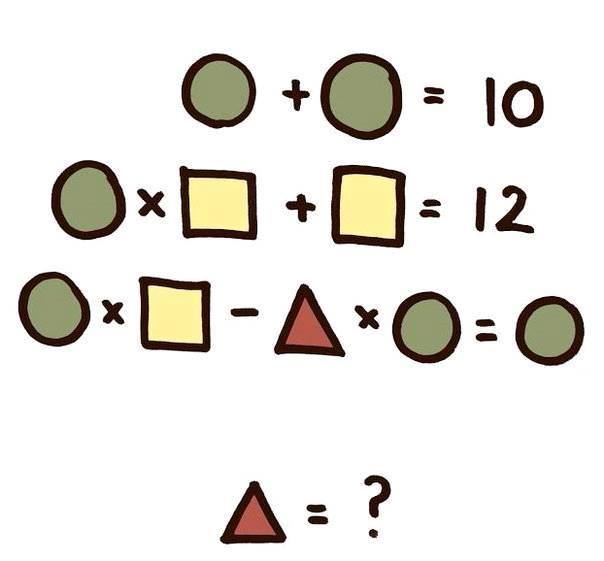
\includegraphics[scale=0.3]{basics/equation.jpg}
\caption{System of equations}
\end{figure}

It's that easy to solve it in Z3:

\begin{lstlisting}
#!/usr/bin/python
from z3 import *

circle, square, triangle = Ints('circle square triangle')
s = Solver()
s.add(circle+circle==10)
s.add(circle*square+square==12)
s.add(circle*square-triangle*circle==circle)
print s.check()
print s.model()
\end{lstlisting}

\begin{lstlisting}
sat
[triangle = 1, square = 2, circle = 5]
\end{lstlisting}

\subsection{Why variables are declared using declare-fun?}

They mean this is nullary function, only returning a constant, nothing else.

\subsection{Connection between \ac{SAT} and \ac{SMT} solvers}

\ac{SMT}-solvers are frontends to \ac{SAT} solvers, i.e.,
they translating input SMT expressions into \ac{CNF} and feed SAT-solver with it.
Translation process is sometimes called ``bit blasting''.
Some \ac{SMT}-solvers uses external SAT-solver: STP uses MiniSAT or CryptoMiniSAT as backend.
Some other \ac{SMT}-solvers (like Z3) has their own SAT solver.

\iffalse
\subsection{Theories}

...

QF\_S -- strings. You may need this to simulate strings to catch bugs like SQL injection.
\url{http://cvc4.cs.stanford.edu/wiki/Strings}.
\fi

% subsubsections:
\subsection{List of SMT-solvers}

\begin{itemize}

\item Yices\footnote{\url{http://yices.csl.sri.com/}}, created by Bruno Dutertre et al.

\item Z3\footnote{\url{https://github.com/Z3Prover/z3}},
developed by Leonardo de Moura, Nikolaj Bjorner, Christoph M. Wintersteiger, Lev Nachmanson.

Many examples here uses Python 2.x API for Z3 (AKA Z3Py).
Installation instructions (Ubuntu):

\begin{lstlisting}
sudo apt-get install python3-pip
sudo pip3 install z3-solver
\end{lstlisting}

Or compile the latest on Ubuntu:

\begin{lstlisting}
git clone https://github.com/Z3Prover/z3.git
cd z3
git tag
git checkout z3-4.8.4	# or another version
python scripts/mk_make.py --python
cd build
make
sudo make install
\end{lstlisting}

(Unofficial) bindings:
Haskell\footnote{\url{http://hackage.haskell.org/package/z3}},
Racket\footnote{\url{https://github.com/philnguyen/z3-rkt}},
Ruby\footnote{\url{https://github.com/prove-rs/z3.rs}}.

\item STP\footnote{\url{https://github.com/stp/stp}}, used in KLEE.

\item CVC3/CVC4\footnote{\url{http://cvc4.stanford.edu/}}.

\item Boolector\footnote{\url{http://fmv.jku.at/boolector/}}, developed by Aina Niemetz, Mathias Preiner and Armin Biere.
Known to be fastest bitvector solver.

\item Alt-Ergo\footnote{\url{https://alt-ergo.ocamlpro.com/}}, used in Frama-C.

\item MathSAT\footnote{\url{http://mathsat.fbk.eu/}}. Developed by Alberto Griggio, Alessandro Cimatti and Roberto Sebastiani.

\item veriT\footnote{\url{http://www.verit-solver.org/}}.
Developed by David Déharbe, Pascal Fontaine, Haniel Barbosa.
Lacks bitvectors.

\item toysolver\footnote{\url{https://github.com/msakai/toysolver}} by Masahiro Sakai, written in Haskell.

\item MK85\footnote{\url{https://github.com/DennisYurichev/MK85}}.
Created by Dennis Yurichev, as a toy bit-blaster, supports booleans and bitvectors.

\item dReal: ``An SMT Solver for Nonlinear Theories of the Reals''
\footnote{\url{http://dreal.cs.cmu.edu}, \url{https://github.com/dreal}}.

\end{itemize}

Something else:

\begin{itemize}

\item PySMT: unified Python interface to many SMT solvers: \url{https://pysmt.readthedocs.io/en/latest/}

\item JavaSMT -- Unified Java API for SMT solvers: \url{https://github.com/sosy-lab/java-smt}

\item jSMTLIB -- Another Java API for SMT solvers: \url{http://smtlib.github.io/jSMTLIB/}

\item SBV: SMT Based Verification in Haskell: \url{http://leventerkok.github.io/sbv/}

\end{itemize}


\subsection{Z3 specific}

The output is not guaranteed to be random.
You can randomize it by:

\begin{lstlisting}
import time

...

s=Solver()
set_param("smt.random_seed", int(time.time()))
\end{lstlisting}

Or conversely, you may want to reproduce its result each time the same:

\begin{lstlisting}
set_param("smt.random_seed", 1234)
\end{lstlisting}


